
\documentclass[letterpaper,notitlepage,twoside]{article}

% Basic imports, increase margins...
\usepackage[margin=0.75in]{geometry}
% Finite State Machine stuff
\usepackage{pgf}
\usepackage{tikz}
\usetikzlibrary{arrows, automata}
% Format tables nicely
\usepackage[latin1]{inputenc}
\usepackage{array}

\usepackage{amsfonts}
\usepackage{amssymb}
\usepackage{amsmath,amsthm}

\usepackage{algorithm}          %  float wrapper for algorithms.
\usepackage{algpseudocode}      % layout for algorithmicx

\renewcommand{\implies}{\Rightarrow} % redefine command "implies"
\renewcommand{\iff}{\Leftrightarrow} % double arrow
\newcommand{\maps}{\rightarrow} % define command "map"
\newcommand{\union}{\cup}
\newcommand{\intersect}{\cap}
\newcommand{\N}{\mathbb{N}} % natural number
\newcommand{\Q}{\mathbb{Q}} % rational number
\newcommand{\R}{\mathbb{R}} % real number
\newcommand{\Z}{\mathbb{Z}} % integers
\newcommand\tab[1][1cm]{\hspace*{#1}} %\tab command

% Add more packages that you use here...

\begin{document}
\title{Homework 30}
\author{Brian Knotten, Brett Schreiber, Brian Falkenstein}
\maketitle

\section*{12}
In the CREW algorithm, the concurrent read step is $D[i,j] \gets min(D[i, j], D[i, m] + D[m, j])$, since processor $i = 5$ is reading $D[i = 5, m = 4]$ at the same time processor $j = 4$ is reading $D[m = 5, j = 4]$ (These represent the same memory location). To make the algorithm EREW, make $n$ copies of $D$ into a 3D array $D'$ so that each of the $n^3$ processors $p_{i, j, k}$ is reading from a different cell in $D'$.
\\\\
$n^3$ processors can make $n$ copies of $D$ (which is size $n^2$) into a 3D array $D'$ in $\log^2 n$ time.
\\\\
With $n^3$ processors, the concurrent read step of the CREW algorithm becomes an exclusive read step: $D[i, j, k] \gets min(D[i, j, k], D[i, m, k] + D[m, j, k])$. But now each $D[i, j, k]$ must be synchronized over all $k$, since any one of the $k$s could have changed the minimum. So an extra step must be added to synchronize $D[i, j, k]$ for all $k$.

\section*{13}
The algorithm can be modified as follows to return the actual paths. First, when setting up the 2D array $D$ that contains information for all pairs $(v_i, v_j) \in G$, instead of storing the distance between $v_i$ and $v_j$ store a pair: the first element is a list of vertices representing a path from $v_i$ to $v_j$, and the second element is the distance between $v_i$ and $v_j$.
\\\\
When setting up $D$ initially, $D[i, j]$ is initialized as follows: if $i = j$, then $D[i, j] \gets ([v_i], 0)$. Else if there is an edge between $v_i$ and $v_j$, then $D[i, j] \gets ([v_i, v_j], edge_weight(v_i, v_j))$. Otherwise, $D[i, j] \gets ([], \infty)$.
\\\\
When $D[i, j]$ is updated to be $D[i, m] + D[m, j]$, then $D[i, j] \gets (fst(D[i, m]) ++ fst(D[m, j]), snd(D[i, m]) + snd(D[m, j]))$, where $fst$ returns the first element of a tuple, $snd$ returns the second element of a tuple, and $a ++ b$ represents list $a$ concatenated with list $b$.

\section*{14}
The main idea of this algorithm is to convert the input of longest common subsequence (referred to as LCS) to the input for all-pairs shortest path (APSP). Because we showed in class a CREW algorithm for APSP that runs in time $log^2n$ with a polynomial number of processors, if we can do the input conversion in $log^2n$ time, we can pass the converted input into our APSP algorithm to get our output in $log^2n$ time. \\
Because the CREW algorithm fo APSP has already been extensively defined, this algorithm will focus on the input conversion. The constructed graph will have $N*M = n^2$ nodes, where $N$ and $M$ are the lengths of the input strings to LCS, where node $n_{i j}$ corresponds to the $i'th$ letter in $A$ and the $j'th$ letter in $B$ (if the input strings to LCS are $A$ and $B$). Edges are created according to the following rules:
\begin{itemize}
\item If $A[i] = B[j]$, then add an edge from $n_{ij}$ to $n_{i+1 j+1}$ with weight -1
\item If $A[i] != B[j]$ then add edges from $n_{ij}$ to $n_{i+1j}$ and $n_{ij+1}$ with weights 1
\end{itemize}
Thus the minimum weight path from node $n_{00}$ to $n_{NM}$ will have taken the maximum number of 'diagonal' edges (that is, from $n_{ij}$ to $n_{i+1 j+1}$) as these edges have negative weight and will contribute to the min distance. \\
A simple example of this conversion is provided, where the input strings to LCS are $A=XYYX$ and $B=YZYQ$: 
$$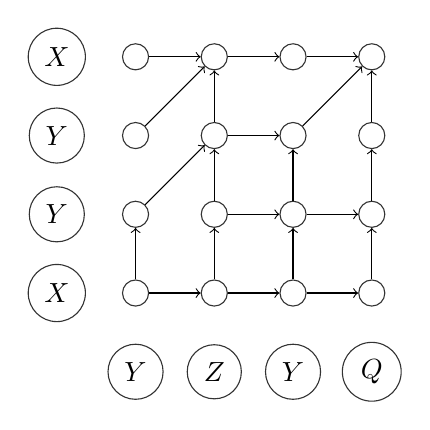
\begin{tikzpicture}
	\node[circle,draw=black!80] (a1) at (0, 1) {$X$};
	\node[circle,draw=black!80] (a2) at (0, 2) {$Y$};
	\node[circle,draw=black!80] (a3) at (0, 3) {$Y$};
	\node[circle,draw=black!80] (a4) at (0, 4) {$X$};
	\node[circle,draw=black!80] (b1) at (1, 0) {$Y$};
	\node[circle,draw=black!80] (b2) at (2, 0) {$Z$};
	\node[circle,draw=black!80] (b3) at (3, 0) {$Y$};
	\node[circle,draw=black!80] (b4) at (4, 0) {$Q$};
	
	\node[circle,draw=black!80] (x1) at (1, 1) {};
	\node[circle,draw=black!80] (x2) at (1, 2) {};
	\node[circle,draw=black!80] (x3) at (1, 3) {};
	\node[circle,draw=black!80] (x4) at (1, 4) {};
	
	\node[circle,draw=black!80] (x5) at (2, 1) {};
	\node[circle,draw=black!80] (x6) at (2, 2) {};
	\node[circle,draw=black!80] (x7) at (2, 3) {};
	\node[circle,draw=black!80] (x8) at (2, 4) {};
	
	\node[circle,draw=black!80] (x9) at (3, 1) {};
	\node[circle,draw=black!80] (x10) at (3, 2) {};
	\node[circle,draw=black!80] (x11) at (3, 3) {};
	\node[circle,draw=black!80] (x12) at (3, 4) {};
	
	\node[circle,draw=black!80] (x13) at (4, 1) {};
	\node[circle,draw=black!80] (x14) at (4, 2) {};
	\node[circle,draw=black!80] (x15) at (4, 3) {};
	\node[circle,draw=black!80] (x16) at (4, 4) {};

	\path[->] (x1) edge node {} (x5);
	\path[->] (x1) edge node {} (x2);
	\path[->] (x5) edge node {} (x9);
	\path[->] (x5) edge node {} (x6);
	\path[->] (x9) edge node {} (x13);
	\path[->] (x9) edge node {} (x10);
	\path[->] (x13) edge node {} (x14);
	
	\path[->] (x2) edge node {} (x7);
	\path[->] (x6) edge node {} (x10);
	\path[->] (x6) edge node {} (x7);
	\path[->] (x10) edge node {} (x14);
	\path[->] (x10) edge node {} (x11);
	\path[->] (x14) edge node {} (x15);
	
	\path[->] (x3) edge node {} (x8);
	\path[->] (x7) edge node {} (x11);
	\path[->] (x7) edge node {} (x8);
	\path[->] (x11) edge node {} (x16);
	\path[->] (x15) edge node {} (x16);
	
	\path[->] (x4) edge node {} (x8);
	\path[->] (x8) edge node {} (x12);
	\path[->] (x12) edge node {} (x16);
\end{tikzpicture}$$
In this picture, the edges with weight -1 are the diagonals, while all horizontal/vertical edges have weight 1. Its important to note that this constructs a graph with no cycles of negative aggregate weight. This is because in any cycle, there will be more positive weighted edges than negatives. With $n^2$ processors, where each processor is assigned an $i, j$, an algorithm is given: 
\begin{algorithm}
\begin{algorithmic}%[1]
\caption{CRCW O(1) algorithm for computing input from LCS to input for APSP}
\Require 2 Strings A and B of size $N$ and $M$, a processor $p_{ij}$ and an adjacency matrix Adj of size $NM\times NM$ 
\If{A[i] ==B[j]}
\State $Adj[i+1][j+1] \gets -1$ \Comment{Negative edge weight, because we found a candidate character for the LCS}
\Else
\State $Adj[i+1][j] \gets 1$ \Comment{Positive edge weight, not part of the LCS}
\State $Adj[i][j+1] \gets 1$
\EndIf
\end{algorithmic}
\end{algorithm}
This construction takes constant time, as each processor simply compares 2 characters and makes either 1 or 2 writes. Also note that because $i, j$ are unique for each processor, this algorithm is exclusive write. \\
Once we have the adjacency matrix constructed, we can simply pass it into the defined algorithm for APSP. \\
Since the input transformation takes constant time, and time for APSP with $p=O(n)$ is $log^2n$, our algorithm also runs in time $log^n$ with $p=O(n)$ processors. 
\end{document}
